The following steps can be carried out at any point during specification, 
 but must be carried out before object mapping, observation or testing begins. 

\begin{enumerate}
\item Select the \gdserver you want to start from the drop-down menu next to the  \bxcaption{Connect to \gdserver} button on the toolbar (\bxfigref{TutConnectServer}). 
\begin{figure}[h]
\begin{center}
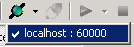
\includegraphics{Tutorials/PS/TutConnectServer}
\caption{Connect to \gdserver}
\label{TutConnectServer}
\end{center}
\end{figure}

\item In the status bar in the bottom right-hand corner of the perspective, you can see the \gdserver status. 
\item Select the \gdaut{} and configuration you want to start from the drop-down menu next to the  \bxcaption{Start \gdaut{}} button on the toolbar (\bxfigref{TutStartAUT}).
\begin{figure}[h]
\begin{center}
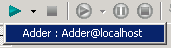
\includegraphics{Tutorials/PS/TutStartAUT}
\caption{Start the \gdaut{}}
\label{TutStartAUT}
\end{center}
\end{figure}

\item The \gdaut{} will appear,and the  status 
bar will change to show the new status. 
\item Depending on the system 
configuration, the Adder may be hidden behind some other window. Bring the 
Adder to the front to continue. 
\end{enumerate}
